\documentclass[10pt]{article}
\usepackage[margin=0.9in]{geometry}
\usepackage{amsmath,amssymb,graphicx,booktabs,hyperref,microtype}
\usepackage[T1]{fontenc}
\usepackage{lmodern}
\graphicspath{{../figures/}}
\hypersetup{colorlinks=true,urlcolor=blue,linkcolor=blue,citecolor=blue}
\newcommand{\Om}{\Omega}
\title{Stability windows of the Golden Pancake three-body isola:\\
Krein collisions, a half-period reflection symmetry and outer-mass sensitivity}
\author{Yuanqing Liu \and Han Liu \and Anqing Xuan}
\date{Draft, 12 October 2026}
\begin{document}
\maketitle
\begin{abstract}
The \emph{Golden Pancake Drama} orbits are planar, collisionless, zero-angular-momentum periodic
solutions of the Newtonian three-body problem with masses $(1,\mu,1)$, recently reported by the
Three Body Orbits atlas on a closed isola $0.4689\lesssim\mu\lesssim0.6346$; the atlas asserts
linear stability for one representative ($\mu\simeq0.61236$). We map the planar linear (spectral)
stability along the isola. On the segment containing the stable representative we find three
spectrally stable stretches, bounded by four transversal Krein collisions of opposite-signature
multipliers and by the fold at $\mu_{\max}$. The edges of the main window are
$\mu_L=0.59904378420889985122072886046\ldots$ and
$\mu_R=0.61784426820906317872736671060\ldots$ (Table~\ref{tab:trans}); two independent multiprecision
pipelines (MPFR Taylor and Gragg--Bulirsch--Stoer integrators with separate shooting and Floquet
codes) agree to about 60 significant digits. Near both edges the colliding multipliers split as
$|\mu-\mu_\ast|^{1/2}$ and the monodromy has a $2\times2$ Jordan block at the collision, the linear
signature of a Hamiltonian--Hopf bifurcation. Every orbit on the isola satisfies a half-period
reflection symmetry, so the monodromy is a square; this explains why multipliers touch $-1$
without crossing it (at 1:4 resonances of the half-period map), with no change of spectral
stability; possible nonlinear bifurcations there are not investigated. For outer masses
$(1+\delta,\mu,1-\delta)$ the orbits remain exactly periodic and the main window closes at
$|\delta|\approx0.0086$. Our orbit at the atlas's 42-digit mass agrees with its published initial
conditions to $10^{-36}$--$10^{-38}$. All statements are numerical evidence, not
computer-assisted proofs.
\end{abstract}

\section{Introduction}
Large numerical searches have produced thousands of planar periodic three-body orbits with zero
angular momentum, including many unequal-mass families
\cite{suvakov2013,lili2017,lijingliao2018,lililiao2021,hristov2024,hristov2026}. Whether a periodic
orbit is linearly stable, and how stability changes along a family as the masses vary, has been
studied for the figure-eight \cite{galan2002,simo2002,kapela2007} and, statistically, across the
published catalogues \cite{dmitrasinovic2018,vasiljevic2023}. The Three Body Orbits atlas
recently reported the \emph{Golden Pancake Drama} family, an isola of orbits with masses
$(1,\mu,1)$ in the Euler-half-twist sector, and found one linearly stable representative at
$\mu=0.612356088827994835\ldots$; its draft note states that ``only the marked orbit's linear
stability is asserted'' \cite{atlasnote,atlas}. The present note locates and classifies the
stability transitions along that isola. The family is not new; its stability structure is the
subject here.

\section{Model and numerical methods}
We integrate $\ddot{\mathbf q}_i=\sum_{j\ne i}m_j(\mathbf q_j-\mathbf q_i)/\|\mathbf q_j-\mathbf q_i\|^3$,
$G=1$, $(m_1,m_2,m_3)=(1,\mu,1)$, from the Euler section
$\mathbf q_{1,2,3}=(-1,0),(0,0),(1,0)$, $\dot{\mathbf q}_1=\dot{\mathbf q}_3=(u,v)$,
$\dot{\mathbf q}_2=-2(u,v)/\mu$, which fixes the centre of mass, zero momentum and $L=0$
\cite{atlasnote}. Periodic orbits solve $X(T)-X(0)=0$ for all twelve labelled positions and
velocities by least-squares Newton in $(u,v,T)$; no rotation or body permutation is allowed.

\textbf{Two independent multiprecision pipelines.} (i) An adaptive Taylor integrator in MPFR with
Decimal shooting and a symplectic-quotient Floquet reduction; (ii) a Gragg--Bulirsch--Stoer
extrapolation integrator in MPFR (modified midpoint rule, step sequence $2j$, Aitken--Neville
extrapolation in $h^2$), mpmath shooting from binary64 seeds, and a reduction-free Floquet
analysis. The two share no integration, shooting or spectral code. In (ii), because the eight
trivial multipliers of the exact monodromy $\Phi$ equal $1$, the nontrivial quartic follows from
$p_k=\operatorname{tr}\Phi^k-8$ ($k\le4$) by Newton's identities; with pair sums
$s=\lambda+\lambda^{-1}$ solving $s^2-p_1s+(e_2-2)=0$, the discriminant is
$D=2p_2+8-p_1^2=(s_1-s_2)^2$. Spectral stability holds iff both $s_i$ are real and in $(-2,2)$;
$D<0$ signals a complex quartet. Krein forms $\kappa=\operatorname{Re}(i\,z^{\mathsf H}\Om z)$ use
full-space eigenvectors and $\Om=\bigl(\begin{smallmatrix}0&M\\-M&0\end{smallmatrix}\bigr)$,
$M=\operatorname{diag}(1,1,\mu,\mu,1,1)$. Typical settings: 80--90 digits, final closures
$10^{-62}$--$10^{-65}$, verification runs with stricter tolerances than the Newton runs.
Transitions are refined by secant iteration on $D$ (or $q(\pm1)=\prod_i(\pm1-\lambda_i)$ for
$s=\pm2$ crossings), each evaluation being a fresh Newton-corrected orbit; the sign of the
transition function is then verified at $\mu_\ast\mp10^{-30}$. Binary64 pseudo-arclength
continuation in $(u,v,T,\mu)$, with an exact mass-sensitivity column, maps the whole isola.

\textbf{Validation.} On common orbits the pipelines agree to $|\Delta D|\approx5\times10^{-59}$
and $|\Delta\Phi|\approx10^{-60}$. Continuing our own branch to the atlas's 42-digit mass gives
$(u,v,T)$ differing from the atlas's Table~1 \cite{atlasnote} by $3.3\times10^{-38}$,
$1.9\times10^{-38}$ and $1.5\times10^{-36}$ (the atlas states a closure of $1.5\times10^{-36}$),
and multipliers agreeing with its 19-digit values to $4\times10^{-20}$. The largest nontrivial
multiplier moduli of the two other atlas orbits on this branch ($\mu=0.58764$, $0.63031$) are
$1.16366$ and $2.38147$, reproducing the catalogue values $1.1637$ and $2.3815$ \cite{atlas}.

\section{Results}
\textbf{Stability along the isola.} Figure~\ref{fig:overview} shows the isola in the $(u,\mu)$
plane and the pair sums along the AABAbbaabaBB segment, which contains the atlas
representative. Three stretches are spectrally stable: from the end of our scan
($\mu\approx0.5393$, where the binary64 corrector reaches its accuracy limit before the collision
limit near $\mu\approx0.5066$) up to $K_0$; the main window $[K_1,K_2]$; and a narrow stretch
$[K_3,\mu_{\max}]$ next to the fold, where a multiplier pair passes $+1$
($\mu_{\max}\approx0.6346043$ from our scan, $0.6346042508$ in \cite{atlasnote}). The
$(ABab)^3$ segment is unstable except for a short stretch beyond its $\mu_{\min}$ fold, starting
at an $s=+2$ crossing $T_1$ at $\mu=0.475901444\ldots$. Table~\ref{tab:trans} lists the refined
transitions; every crossing is transversal.

\begin{figure}[t]
\centering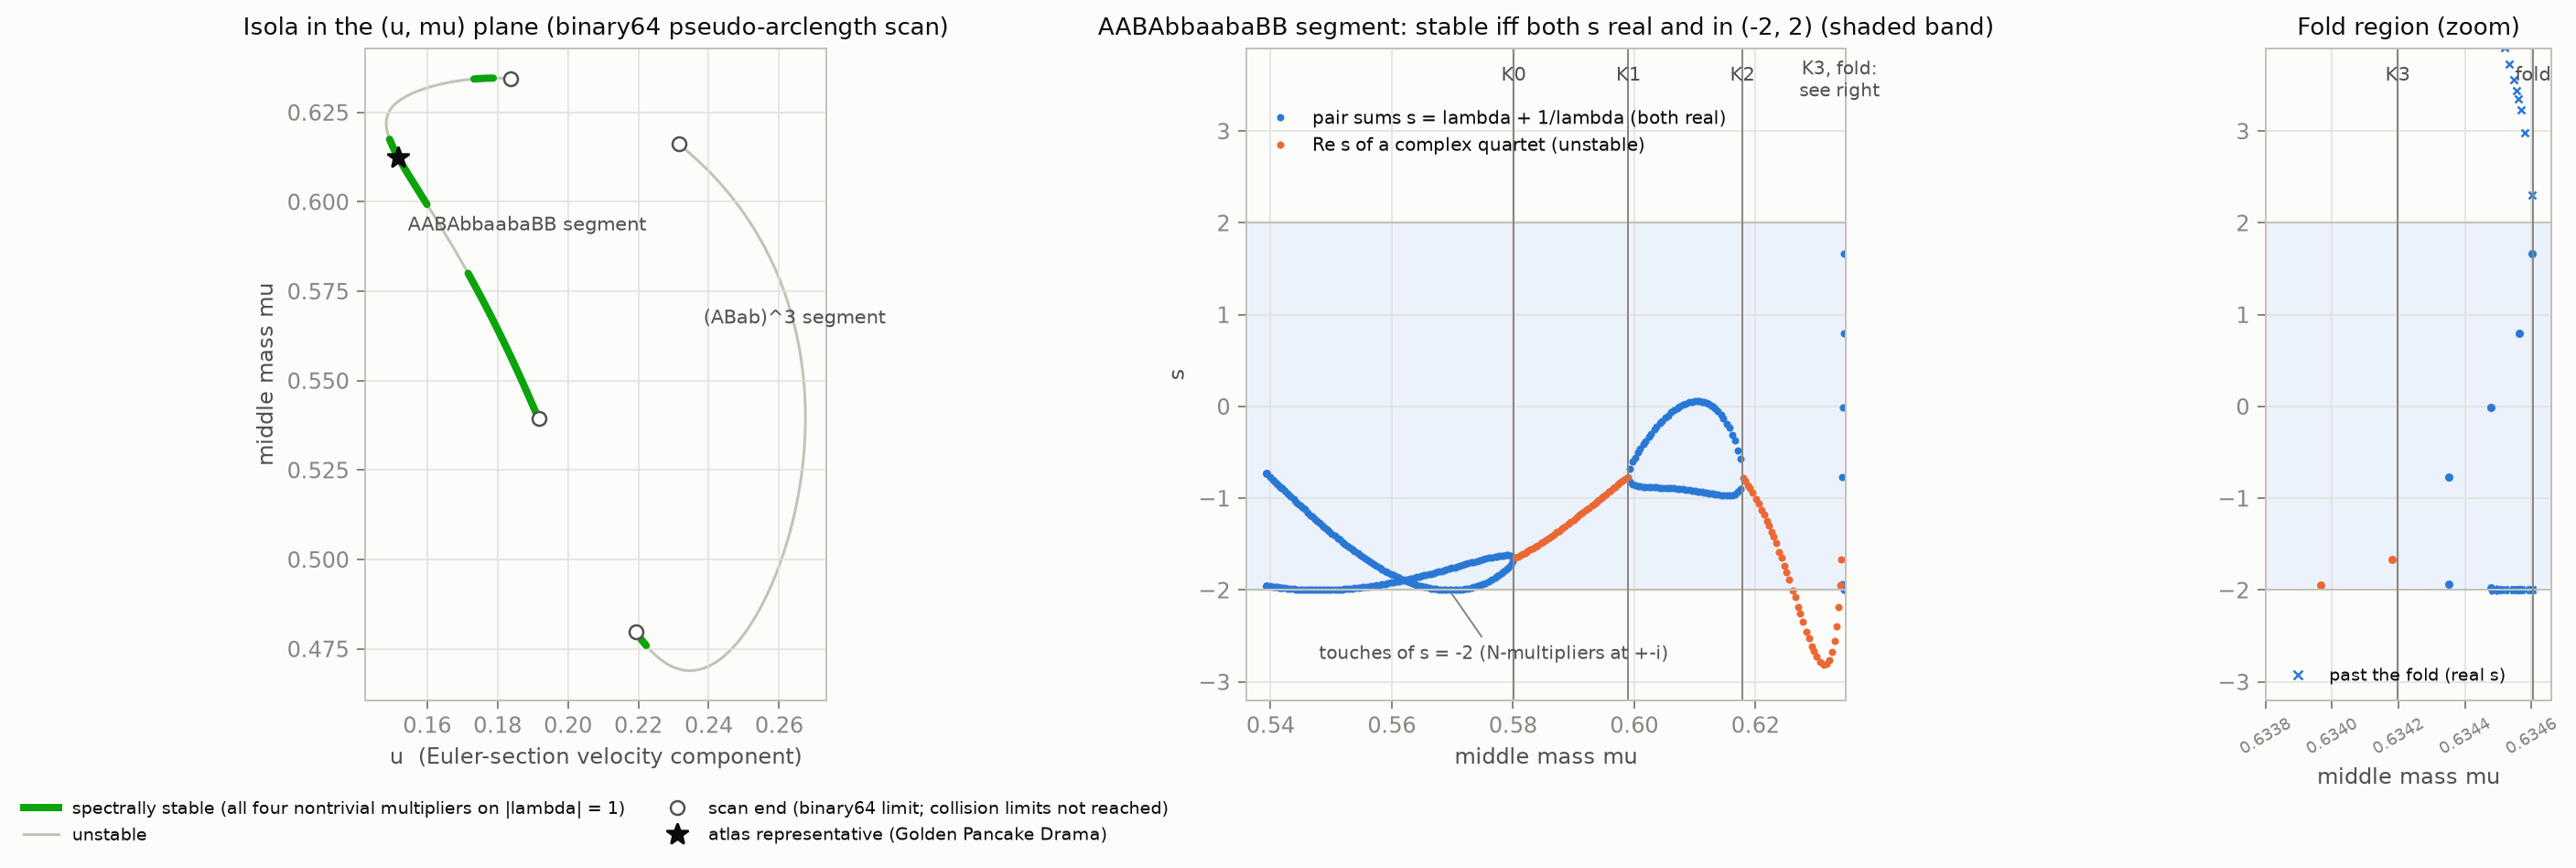
\includegraphics[width=\linewidth]{isola_stability_overview.png}
\caption{Left: the isola (binary64 pseudo-arclength scan); green, spectrally stable; open
circles, ends of the scans before the collision limits; star, atlas representative. Centre:
pair sums $s=\lambda+\lambda^{-1}$ on the AABAbbaabaBB segment; blue, both real; orange, real part
of a complex quartet. Right: the fold region.}\label{fig:overview}
\end{figure}

\begin{table}[t]
\centering\small
\caption{Spectral transitions. Digits are truncated where the two independent implementations
(Taylor and GBS) agree, excluding each run's last printed digit; all
listed transitions have verified sign changes of the transition function at $\mu_\ast\mp10^{-30}$.}
\label{tab:trans}
\begin{tabular}{@{}llll@{}}\toprule
 & type & $\mu_\ast$ & $\mathrm d D/\mathrm d\mu$\\\midrule
$K_0$ & Krein & $0.580094414288468996548897180964879640274\ldots$ & $-22.25$\\
$K_1=\mu_L$ & Krein, Jordan & $0.599043784208899851220728860462068419275413725661780425744347\ldots$ & $+74.87$\\
$K_2=\mu_R$ & Krein, Jordan & $0.617844268209063178727366710600417996702072689168837458676169\ldots$ & $-305.9$\\
$K_3$ & Krein & $0.634197066930554588552605424098150004643\ldots$ & $+5840$\\
fold & $s=+2$ & $\approx0.6346043$ (binary64) & ---\\
$T_1$ & $s=+2$, $(ABab)^3$ & $0.475901444550864118752069986423460087896\ldots$ & ---\\\bottomrule
\end{tabular}
\end{table}

\textbf{Type of the main transitions.} At $K_1$ and $K_2$ the two colliding multipliers have
opposite Krein signatures. Sampling $\mu=\mu_\ast\pm10^{-k}$, $4\le k\le40$, at 80 digits
(Fig.~\ref{fig:scaling}) gives on the stable side $|\lambda_1-\lambda_2|\propto\delta^{0.5000}$
and normalized Krein forms $\propto\delta^{0.501}$, on the unstable side
$|\lambda|-1\propto\delta^{0.5000}$, and eigenvector non-overlap $\propto\delta^{1.000}$. At
$\mu_\ast$ the smallest singular value of $\Phi-\bar\lambda I$ is $3\times10^{-61}$ ($K_1$) and
$2\times10^{-62}$ ($K_2$) while the next is $0.020$ and $0.092$: the collision eigenvalue has
geometric multiplicity one and algebraic multiplicity two. This is the linear part of a
Hamiltonian--Hopf bifurcation \cite{vandermeer1985,howard1987}; we have not computed the
nonlinear normal-form coefficient that distinguishes its super- and subcritical cases.

\begin{figure}[t]
\centering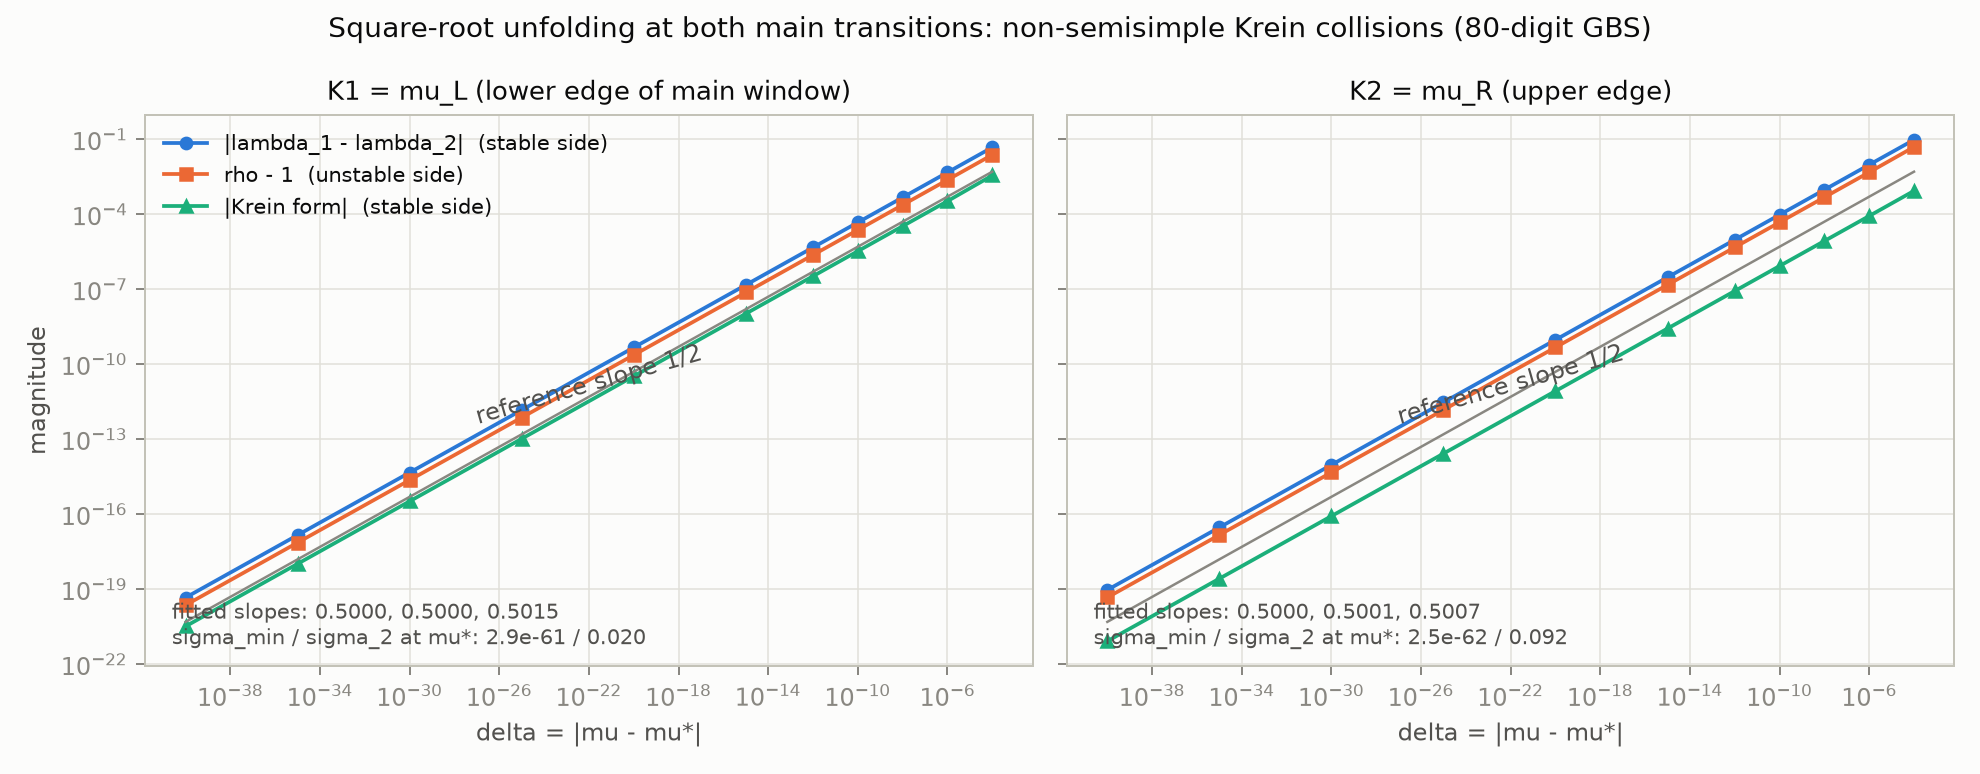
\includegraphics[width=0.95\linewidth]{transition_scaling.png}
\caption{Square-root unfolding of the Krein collisions $K_1$ and $K_2$ (80-digit GBS orbits).}
\label{fig:scaling}
\end{figure}

\textbf{Half-period reflection symmetry.} The atlas computes this family in an
``Euler-half-twist'' symmetric sector with half-period shooting \cite{atlasnote}; we make the
symmetry and its spectral consequences explicit. For every orbit computed, $X(T/2)=\sigma X(0)$ where
$\sigma$ reflects all positions and velocities across a line through the centre of mass (defect
$\le8\times10^{-63}$ at 80 digits; the axis angle varies with $\mu$). Since reflections commute
with the Newtonian flow, $X(t+T/2)=\sigma X(t)$ and $\Phi=N^2$ with
$N=\sigma\,\mathrm D\varphi_{T/2}(X(0))$; numerically $|N^2-\Phi|\le3.3\times10^{-59}$. Hence
$s_\Phi=s_N^2-2\ge-2$ for real $s_N$: a pair of multipliers of $\Phi$ can reach $-1$ only
tangentially, when a pair of $N$ passes $\pm i$, i.e.\ at a 1:4 resonance of $N$. The scan shows
exactly this near $\mu\approx0.5695$ and $0.5481$; the multipliers of $\Phi$ stay on the unit
circle, so spectral stability does not change there. The statement is spectral only: 1:4
resonances generically create period-4 orbits of the resonant map, including non-symmetric ones
born in pitchfork bifurcations \cite{gonchenko2018}, which here would be period-$2T$ orbits of the
flow breaking the half-period symmetry; we have not investigated such nonlinear bifurcations. A
further near-coincidence near $\mu\approx0.5619$ is a pass-through of pairs of equal Krein sign,
again without a spectral change. The discriminant of $N$ changes sign at $K_1$ and $K_2$ together
with that of $\Phi$, so these are collisions of the half-period map itself.

\textbf{Unequal outer masses.} For masses $(1+\delta,\mu,1-\delta)$ we replace the symmetric
ansatz by a general collinear section with zero momentum and $L=0$ and solve
$X(T)=R_\theta X(0)$ with the rotation angle $\theta$ as an unknown. The solutions remain exactly
periodic ($|\theta|\le4\times10^{-11}$ in binary64), as the persistence of the reflection
symmetry for arbitrary masses suggests. The main window narrows quadratically,
$\mu_L(\delta)\approx\mu_L+126\,\delta^2$, $\mu_R(\delta)\approx\mu_R-39\,\delta^2$, and closes at
$|\delta|\approx0.0086$ near $\mu\approx0.611$ (Fig.~\ref{fig:asym}). The scan is binary64 and
symmetric under $\delta\to-\delta$ to $3\times10^{-11}$.

\begin{figure}[t]
\centering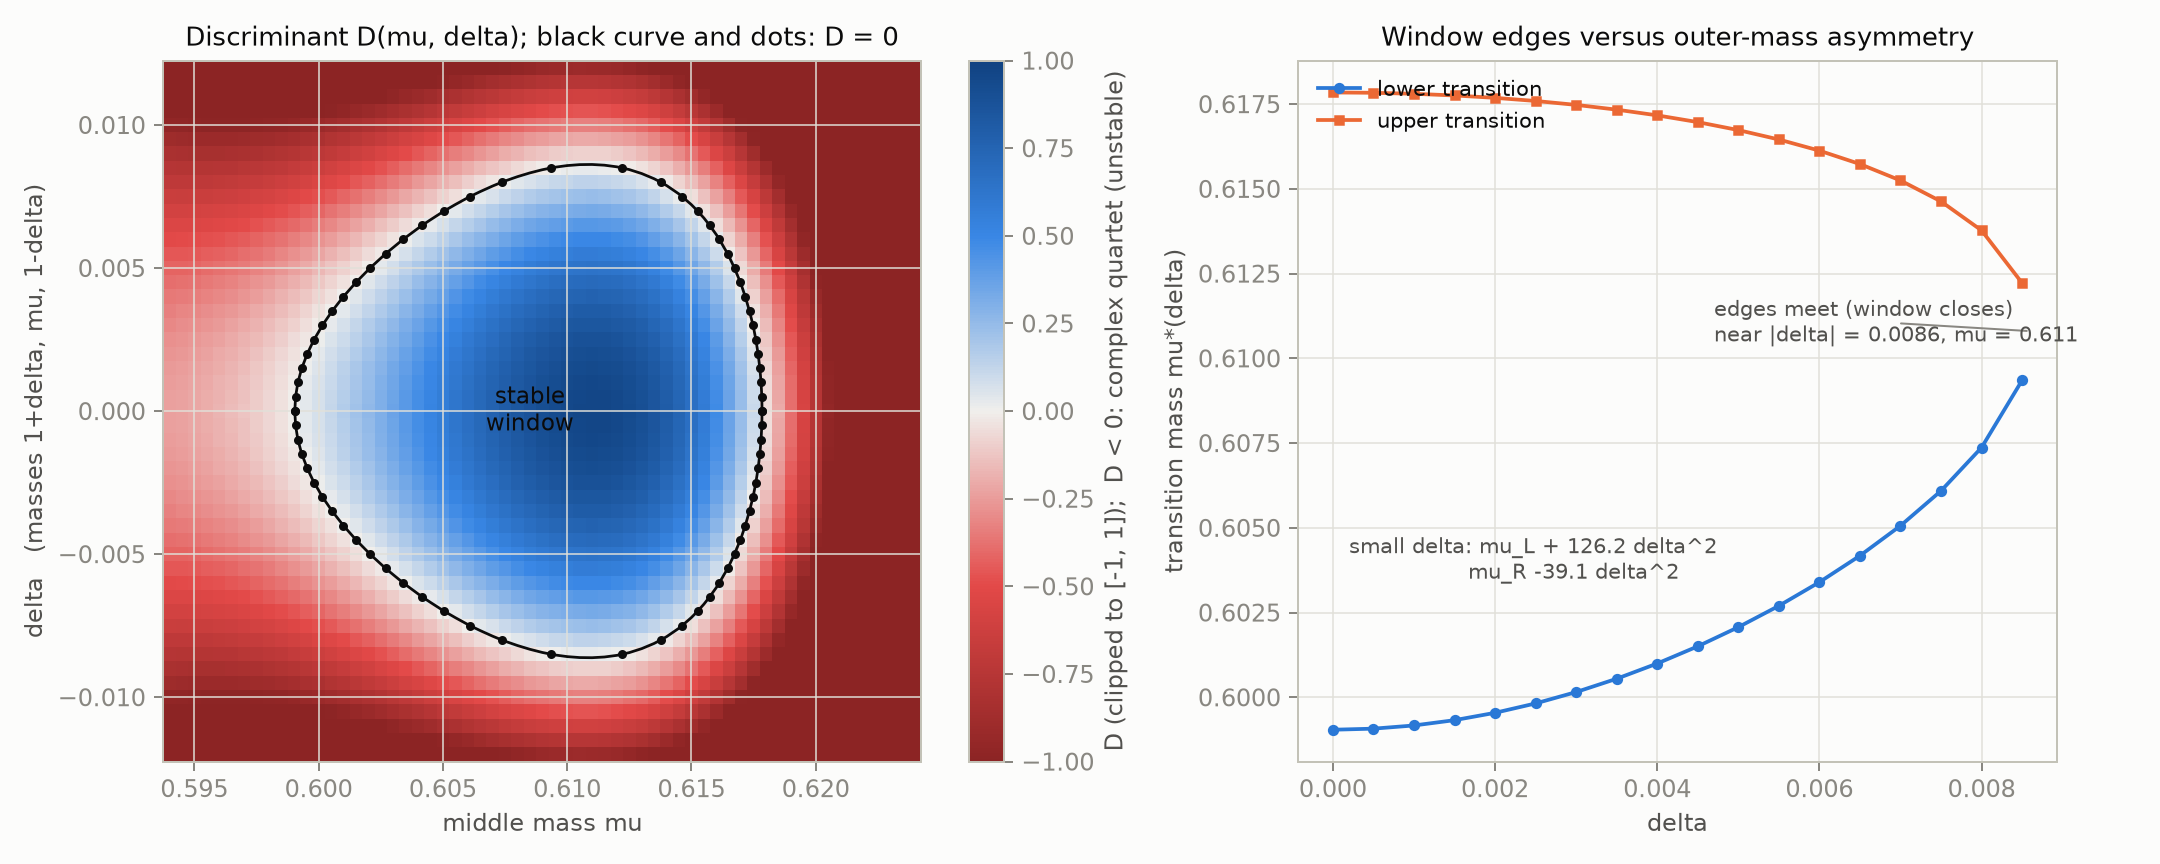
\includegraphics[width=0.95\linewidth]{asymmetric_stability_region.png}
\caption{Left: discriminant $D(\mu,\delta)$ for masses $(1+\delta,\mu,1-\delta)$ (binary64);
the black curve is $D=0$ and bounds the stable window. Right: window edges versus $\delta$.}
\label{fig:asym}
\end{figure}

\section{Discussion and limitations}
The main stability window of the Golden Pancake isola is bounded by Hamiltonian--Hopf-type
Krein collisions, and stable motion survives on two further stretches of the same segment.
The window is narrow in the outer-mass asymmetry ($|\delta|\lesssim0.009$), wider than the
$10^{-5}$-scale stability region reported for the figure-eight \cite{lililiao2021} but far
narrower in $\delta$ than in $\mu$. The evidence is numerical: closures and spectra are confirmed
by independent integrators, precisions and the atlas's own data, but nothing here is an
interval-arithmetic proof of existence or of the spectral statements (compare \cite{kapela2007});
local error control is heuristic; the binary64 scans can miss features finer than their step and
stop before the binary-collision limits; and only spectral stability is addressed --- nonlinear
phenomena, such as orbits bifurcating at the 1:4 resonances of the half-period map or the
normal-form type of the Hamiltonian--Hopf transitions, are not.

\paragraph{Data and code.} Scripts, raw multiprecision trajectories and monodromy matrices,
logs, source snapshots and tests accompany this draft (project repository, \texttt{README.md}).

\begin{thebibliography}{99}\small
\bibitem{atlasnote} Three Body Orbits, ``golden pancake drama: a linearly stable three-body orbit on an unequal-mass isola,'' draft numerical research note, 9 September 2026, \url{https://www.threebodyorbits.com/papers/golden-pancake-drama-2026.pdf}.
\bibitem{atlas} Three Body Orbits atlas, family page and catalogue, \url{https://www.threebodyorbits.com/family/golden-pancake-drama}, \url{https://data.threebodyorbits.com/catalogue.json} (accessed 12 October 2026).
\bibitem{suvakov2013} M. \v{S}uvakov and V. Dmitra\v{s}inovi\'c, Phys. Rev. Lett. \textbf{110}, 114301 (2013).
\bibitem{lili2017} X. Li and S. Liao, Sci. China Phys. Mech. Astron. \textbf{60}, 129511 (2017).
\bibitem{lijingliao2018} X. Li, Y. Jing and S. Liao, Publ. Astron. Soc. Japan \textbf{70}, 64 (2018).
\bibitem{lililiao2021} X. Li, X. Li and S. Liao, Sci. China Phys. Mech. Astron. \textbf{64}, 219511 (2021).
\bibitem{hristov2024} I. Hristov and R. Hristova, Astron. Comput. \textbf{49}, 100880 (2024).
\bibitem{hristov2026} I. Hristov, R. Hristova and K. Tanikawa, New Astron. \textbf{125} (2026).
\bibitem{galan2002} J. Gal\'an, F. J. Mu\~noz-Almaraz, E. Freire, E. Doedel and A. Vanderbauwhede, Phys. Rev. Lett. \textbf{88}, 241101 (2002).
\bibitem{simo2002} C. Sim\'o, Contemp. Math. \textbf{292}, 209 (2002).
\bibitem{kapela2007} T. Kapela and C. Sim\'o, Nonlinearity \textbf{20}, 1241 (2007).
\bibitem{dmitrasinovic2018} V. Dmitra\v{s}inovi\'c, A. Hudomal, M. Shibayama and A. Sugita, J. Phys. A \textbf{51}, 315101 (2018).
\bibitem{vasiljevic2023} V. Vasiljevi\'c, B. Raoni\'c and V. Dmitra\v{s}inovi\'c, New Astron. \textbf{100}, 101969 (2023).
\bibitem{vandermeer1985} J.-C. van der Meer, \emph{The Hamiltonian Hopf Bifurcation}, Lecture Notes in Mathematics 1160 (Springer, 1985).
\bibitem{howard1987} J. E. Howard and R. S. MacKay, J. Math. Phys. \textbf{28}, 1036 (1987).
\bibitem{gonchenko2018} M. Gonchenko, S. V. Gonchenko, I. Ovsyannikov and A. Vieiro, Chaos \textbf{28}, 043123 (2018), arXiv:1711.09447.
\end{thebibliography}
\end{document}
